Neutrino physics is at the core of current high energy research. One of the profound discoveries made in recent years was the observation of neutrino flavour oscillations by the Super-Kamiokande (Super-K) experiment, which was the first confirmation that physics existed beyond the standard model of particle physics. In brief, neutrinos described by the standard model would be massless particles, but since the flavours are made up of superpositions of mass states, the oscillation of
the flavour states implies that the relative mass states are different, and therefore non-zero \cite{nuInt}.

    Future, long-baseline,  neutrino experiments such as the Deep Underground Neutrino Experiment (DUNE) and Hyper-Kamiokande (Hyper-K) are hoping to investigate some of the most fundamental questions we are still asking: Why does the universe constist of matter, and not anti-matter? What is the neutrino mass heirarchy? Neutrino research is an extremely active field. Optimising the current and future detectors to maximise the accuracy of all interaction anaylses is a crucial step towards obtaining concrete answers to these questions. 

    A brief introduction to the topics covered in this report is as follows, more detail on each will be given in later sections. 

\subsection{Neutrino interactions}

Due to the elusive nature of the neutrino, directly observing one in a detector isn't possible. It is therefore necessary to infer their existence from particles produced when they interact. Since this process relies upon the reconstruction capability of the experiment, purpose-built detectors will attempt to maximise the efficiency of this.

Another property of the neutrino which poses a significant difficulty within detectors is their interaction probability, or cross-section. A typical neutrino cross-section is on the order of $ 10^{-44} $ cm$^{2}$ which corresponds to $\sim$1 interaction every 10 light years in steel, for neutrinos with only a few MeV energy \cite{nuOsc}. This fact introduces the need for the interacting neutrinos to have high energies in these dedicated experiments, if we are to sufficiently reduce their mean free path. More detail on this topic will be discussed in section~\ref{sec:NIP}.

\subsection{GENIE and the GENIE-Professor global fits}

GENIE is the world leading Monte Carlo neutrino interaction generator. Generators are a crucial machinery in all high energy physics analyses as they use theoretical models to produce predictions of how and where neutrino interactions will occur in specific detector geometries \cite{genie}. With this information, comparisons between experimental data and theoretical predictions can be drawn, the models can be improved through fits to such data and potential new physics can be explored. These predictions also help motivate the requirements for building state-of-the art detectors and produce high precision cross-section measurements to improve current and future neutrino physics analyses. 

    An effort to improve model configurations by performing fits to an archive of experimental data is currently being carried out by GENIE using the Professor software framework, which was written with this purpose for experiments at the LHC \cite{prof}. The ultimate goal of this exercise is to perfom a global fit to all neutrino scattering data and consequently produce comprehensive model configurations to further optimise the predictions made for the next generation of neutrino experiments. This work and GENIE's role in current and future neutrino experiments will be discussed further in section~\ref{sec:GF}.

\subsection{Cross-sections}
   
    In order to correctly model neutrino events within a specific detector geometry and material, certain parameters have to be known. In particular, the probability of an interaction taking place - its cross-section - is required for each possible interaction the neutrino could undergo. Cross-section measurements are therefore a necessity for the Monte Carlo event generators, and consequently the future detector studies mentioned earlier. 
    
    The extent of our current knowledge of charged current neutrino cross sections is shown in Figure~\ref{fig:xsecCurr}. The plot contains cross-section information from multiple types of neutrino experiment, differing in both target material and detector machinery. A feature of this plot which is of the most interest to a Short Baseline Near Detector (SBND) cross-section study in particular, is the lack of precision in the measurements made towards the $\sim$1 GeV region
    \cite{xsecCurr}. SBND will not only be operational at this energy range, but it will also have statistics substantial enough to potentially make a significant contribution to improving the current knowledge in this region.

    %CC cross-sections
    \begin{figure}[h!]
        \center
        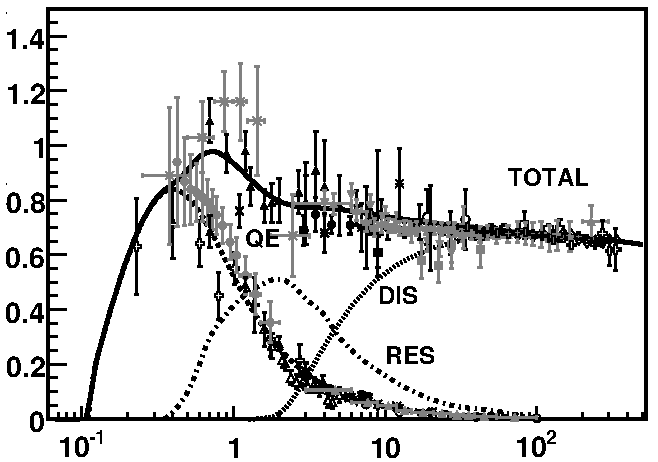
\includegraphics[width=.8\textwidth]{images/current_cross_sec_knowledge.pdf}
        \put(-68, -15){\Large E$_{\nu}$ ( GeV )}
        \put(-375, 50){\Large \rotatebox{90}{$\sigma_{\nu}$ / $\Delta$E$_{\nu}$ ( 10$^{-38}$ cm$^{2}$ / GeV ) }}
        \caption{A compilation of the total cross-section data across the $\sim$1 MeV to $\sim$100 GeV energy range. Including a breakdown in terms of the quasi-elastic, QE, resonant, RES and deep inelastic scattering, DIS, topologies \cite{xsecCurr}. }
        \label{fig:xsecCurr}
    \end{figure}

    The scale of contribution SBND could make to this area of physics would in turn improve the predictions made by event generators for the next generation of neutrino experiments. Cross-sections will be discussed further in section~\ref{sec:XSec}.
    
\subsection{SBND Physics Goals}

SBND is one of 3 liquid argon detectors using the same neutrino beam in the Short Baseline Neutrino (SBN) program. Together, they aim to explore neutrino oscillations at 3 different positions along the beam, allowing for highly senstive measurements to be made \cite{sbn}.   

Another objective of the SBN program, along with many other neutrino physics experiments, is to observe or reject the existence of sterile neutrinos. Though this will not be discussed here.

The MiniBooNE and LSND experiments observed an excess of low energy electron neutrino appearance in their data \cite{mbEx}. One of the main physics goals of SBND is to look for and characterise this excess, in collaboration with any results obtained by the MicroBooNE experiment before SBND is taking data. The beamline of MicroBooNE is 470m compared to 110m for SBND, whether one or both experiments observe the excess will tell us if there was a dependence on the distance travelled by the neutrinos \cite{sbn}. \\

This report will further describe the current status of neutrino cross-section analyses, the level importance that these measurements have in the field, and how a sensitivity calculation in the low GeV energy region is being carried out. It will then explain in more detail how Monte Carlo neutrino generators can be, and are being improved using recent and historical scattering data, through a global fit of comprehensive theoretical model configurations.  

\clearpage
